\documentclass{beamer}
\usepackage{amsmath,graphics}
\usepackage{amssymb}

\usetheme{default}
\usepackage{xcolor}

\definecolor{solarizedBase03}{HTML}{002B36}
\definecolor{solarizedBase02}{HTML}{073642}
\definecolor{solarizedBase01}{HTML}{586e75}
\definecolor{solarizedBase00}{HTML}{657b83}
\definecolor{solarizedBase0}{HTML}{839496}
\definecolor{solarizedBase1}{HTML}{93a1a1}
\definecolor{solarizedBase2}{HTML}{EEE8D5}
\definecolor{solarizedBase3}{HTML}{FDF6E3}
\definecolor{solarizedYellow}{HTML}{B58900}
\definecolor{solarizedOrange}{HTML}{CB4B16}
\definecolor{solarizedRed}{HTML}{DC322F}
\definecolor{solarizedMagenta}{HTML}{D33682}
\definecolor{solarizedViolet}{HTML}{6C71C4}
%\definecolor{solarizedBlue}{HTML}{268BD2}
\definecolor{solarizedBlue}{HTML}{134676}
\definecolor{solarizedCyan}{HTML}{2AA198}
\definecolor{solarizedGreen}{HTML}{859900}
\definecolor{myBlue}{HTML}{162DB0}%{261CA4}
\setbeamercolor*{item}{fg=myBlue}
\setbeamercolor{normal text}{fg=solarizedBase03, bg=solarizedBase3}
\setbeamercolor{alerted text}{fg=myBlue}
\setbeamercolor{example text}{fg=myBlue, bg=solarizedBase3}
\setbeamercolor*{frametitle}{fg=solarizedRed}
\setbeamercolor*{title}{fg=solarizedRed}
\setbeamercolor{block title}{fg=myBlue, bg=solarizedBase3}
\setbeameroption{hide notes}
\setbeamertemplate{note page}[plain]
\beamertemplatenavigationsymbolsempty
\usefonttheme{professionalfonts}
\usefonttheme{serif}

\usepackage{fourier}

\def\vec#1{\mathchoice{\mbox{\boldmath$\displaystyle#1$}}
{\mbox{\boldmath$\textstyle#1$}}
{\mbox{\boldmath$\scriptstyle#1$}}
{\mbox{\boldmath$\scriptscriptstyle#1$}}}
\definecolor{OwnGrey}{rgb}{0.560,0.000,0.000} % #999999
\definecolor{OwnBlue}{rgb}{0.121,0.398,0.711} % #1f64b0
\definecolor{red4}{rgb}{0.5,0,0}
\definecolor{blue4}{rgb}{0,0,0.5}
\definecolor{Blue}{rgb}{0,0,0.66}
\definecolor{LightBlue}{rgb}{0.9,0.9,1}
\definecolor{Green}{rgb}{0,0.5,0}
\definecolor{LightGreen}{rgb}{0.9,1,0.9}
\definecolor{Red}{rgb}{0.9,0,0}
\definecolor{LightRed}{rgb}{1,0.9,0.9}
\definecolor{White}{gray}{1}
\definecolor{Black}{gray}{0}
\definecolor{LightGray}{gray}{0.8}
\definecolor{Orange}{rgb}{0.1,0.2,1}
\setbeamerfont{sidebar right}{size=\scriptsize}
\setbeamercolor{sidebar right}{fg=Black}

\renewcommand{\emph}[1]{{\textcolor{solarizedRed}{\itshape #1}}}

\newcommand\tay{T}
\newcommand\dd{\mathrm d}
\newcommand\eul{\mathrm e}

\newcommand\cA{\mathcal A}
\newcommand\cB{\mathcal B}
\newcommand\cC{\mathcal C}
\newcommand\cD{\mathcal D}
\newcommand\cE{\mathcal E}
\newcommand\cF{\mathcal F}
\newcommand\cG{\mathcal G}
\newcommand\cH{\mathcal H}
\newcommand\cI{\mathcal I}
\newcommand\cJ{\mathcal J}
\newcommand\cK{\mathcal K}
\newcommand\cL{\mathcal L}
\newcommand\cM{\mathcal M}
\newcommand\cN{\mathcal N}
\newcommand\cO{\mathcal O}
\newcommand\cP{\mathcal P}
\newcommand\cQ{\mathcal Q}
\newcommand\cR{\mathcal R}
\newcommand\cS{\mathcal S}
\newcommand\cT{\mathcal T}
\newcommand\cU{\mathcal U}
\newcommand\cV{\mathcal V}
\newcommand\cW{\mathcal W}
\newcommand\cX{\mathcal X}
\newcommand\cY{\mathcal Y}
\newcommand\cZ{\mathcal Z}

\newcommand\fA{\mathfrak A}
\newcommand\fB{\mathfrak B}
\newcommand\fC{\mathfrak C}
\newcommand\fD{\mathfrak D}
\newcommand\fE{\mathfrak E}
\newcommand\fF{\mathfrak F}
\newcommand\fG{\mathfrak G}
\newcommand\fH{\mathfrak H}
\newcommand\fI{\mathfrak I}
\newcommand\fJ{\mathfrak J}
\newcommand\fK{\mathfrak K}
\newcommand\fL{\mathfrak L}
\newcommand\fM{\mathfrak M}
\newcommand\fN{\mathfrak N}
\newcommand\fO{\mathfrak O}
\newcommand\fP{\mathfrak P}
\newcommand\fQ{\mathfrak Q}
\newcommand\fR{\mathfrak R}
\newcommand\fS{\mathfrak S}
\newcommand\fT{\mathfrak T}
\newcommand\fU{\mathfrak U}
\newcommand\fV{\mathfrak V}
\newcommand\fW{\mathfrak W}
\newcommand\fX{\mathfrak X}
\newcommand\fY{\mathfrak Y}
\newcommand\fZ{\mathfrak Z}

\newcommand\fa{\mathfrak a}
\newcommand\fb{\mathfrak b}
\newcommand\fc{\mathfrak c}
\newcommand\fd{\mathfrak d}
\newcommand\fe{\mathfrak e}
\newcommand\ff{\mathfrak f}
\newcommand\fg{\mathfrak g}
\newcommand\fh{\mathfrak h}
%\newcommand\fi{\mathfrak i}
\newcommand\fj{\mathfrak j}
\newcommand\fk{\mathfrak k}
\newcommand\fl{\mathfrak l}
\newcommand\fm{\mathfrak m}
\newcommand\fn{\mathfrak n}
\newcommand\fo{\mathfrak o}
\newcommand\fp{\mathfrak p}
\newcommand\fq{\mathfrak q}
\newcommand\fr{\mathfrak r}
\newcommand\fs{\mathfrak s}
\newcommand\ft{\mathfrak t}
\newcommand\fu{\mathfrak u}
\newcommand\fv{\mathfrak v}
\newcommand\fw{\mathfrak w}
\newcommand\fx{\mathfrak x}
\newcommand\fy{\mathfrak y}
\newcommand\fz{\mathfrak z}

\newcommand\vA{\vec A}
\newcommand\vB{\vec B}
\newcommand\vC{\vec C}
\newcommand\vD{\vec D}
\newcommand\vE{\vec E}
\newcommand\vF{\vec F}
\newcommand\vG{\vec G}
\newcommand\vH{\vec H}
\newcommand\vI{\vec I}
\newcommand\vJ{\vec J}
\newcommand\vK{\vec K}
\newcommand\vL{\vec L}
\newcommand\vM{\vec M}
\newcommand\vN{\vec N}
\newcommand\vO{\vec O}
\newcommand\vP{\vec P}
\newcommand\vQ{\vec Q}
\newcommand\vR{\vec R}
\newcommand\vS{\vec S}
\newcommand\vT{\vec T}
\newcommand\vU{\vec U}
\newcommand\vV{\vec V}
\newcommand\vW{\vec W}
\newcommand\vX{\vec X}
\newcommand\vY{\vec Y}
\newcommand\vZ{\vec Z}

\newcommand\va{\vec a}
\newcommand\vb{\vec b}
\newcommand\vc{\vec c}
\newcommand\vd{\vec d}
\newcommand\ve{\vec e}
\newcommand\vf{\vec f}
\newcommand\vg{\vec g}
\newcommand\vh{\vec h}
\newcommand\vi{\vec i}
\newcommand\vj{\vec j}
\newcommand\vk{\vec k}
\newcommand\vl{\vec l}
\newcommand\vm{\vec m}
\newcommand\vn{\vec n}
\newcommand\vo{\vec o}
\newcommand\vp{\vec p}
\newcommand\vq{\vec q}
\newcommand\vr{\vec r}
\newcommand\vs{\vec s}
\newcommand\vt{\vec t}
\newcommand\vu{\vec u}
\newcommand\vv{\vec v}
\newcommand\vw{\vec w}
\newcommand\vx{\vec x}
\newcommand\vy{\vec y}
\newcommand\vz{\vec z}

\renewcommand\AA{\mathbb A}
\newcommand\NN{\mathbb N}
\newcommand\ZZ{\mathbb Z}
\newcommand\PP{\mathbb P}
\newcommand\QQ{\mathbb Q}
\newcommand\RR{\mathbb R}
\newcommand\RRpos{\mathbb R_{\geq0}}
\renewcommand\SS{\mathbb S}
\newcommand\CC{\mathbb C}

\newcommand{\ord}{\mathrm{ord}}
\newcommand{\id}{\mathrm{id}}
\newcommand{\pr}{\mathrm{P}}
\newcommand{\Vol}{\mathrm{vol}}
\newcommand\norm[1]{\left\|{#1}\right\|} 
\newcommand\sign{\mathrm{sign}}
\newcommand{\eps}{\varepsilon}
\newcommand{\abs}[1]{\left|#1\right|}
\newcommand\bc[1]{\left({#1}\right)} 
\newcommand\cbc[1]{\left\{{#1}\right\}} 
\newcommand\bcfr[2]{\bc{\frac{#1}{#2}}} 
\newcommand{\bck}[1]{\left\langle{#1}\right\rangle} 
\newcommand\brk[1]{\left\lbrack{#1}\right\rbrack} 
\newcommand\scal[2]{\bck{{#1},{#2}}} 
\newcommand{\vecone}{\mathbb{1}}
\newcommand{\tensor}{\otimes}
\newcommand{\diag}{\mathrm{diag}}
\newcommand{\ggt}{\mathrm{ggT}}
\newcommand{\kgv}{\mathrm{kgV}}
\newcommand{\trans}{\top}

\newcommand{\Karonski}{Karo\'nski}
\newcommand{\Erdos}{Erd\H{o}s}
\newcommand{\Renyi}{R\'enyi}
\newcommand{\Lovasz}{Lov\'asz}
\newcommand{\Juhasz}{Juh\'asz}
\newcommand{\Bollobas}{Bollob\'as}
\newcommand{\Furedi}{F\"uredi}
\newcommand{\Komlos}{Koml\'os}
\newcommand{\Luczak}{\L uczak}
\newcommand{\Kucera}{Ku\v{c}era}
\newcommand{\Szemeredi}{Szemer\'edi}

\renewcommand{\ae}{\"a}
\renewcommand{\oe}{\"o}
\newcommand{\ue}{\"u}
\newcommand{\Ae}{\"A}
\newcommand{\Oe}{\"O}
\newcommand{\Ue}{\"U}

\newcommand{\im}{\mathrm{im}}
\newcommand{\rrk}{\mathrm{zrg}}
\newcommand{\crk}{\mathrm{srg}}
\newcommand{\rk}{\mathrm{rg}}
\newcommand{\GL}{\mathrm{GL}}
\newcommand{\SL}{\mathrm{SL}}
\newcommand{\SO}{\mathrm{SO}}
\newcommand{\nul}{\mathrm{nul}}
\newcommand{\eig}{\mathrm{eig}}

\newcommand{\mytitle}{Numerische Quadratur}

\title[Annuma]{\mytitle}
\author[Amin Coja-Oghlan]{Amin Coja-Oghlan}
\institute[Frankfurt]{JWGUFFM}
\date{}

\begin{document}

\frame[plain]{\titlepage}

\begin{frame}\frametitle{\mytitle}
	\begin{block}{Worum geht es?}
		\begin{itemize}
			\item Das Ziel ist, ein Integral $\int_a^bf(x)\dd x$ numerisch zu bestimmen.
			\item Daf\ue r gibt es kein universelles Patentrezept.
			\item Wir werden aber einige ``Quadraturverfahren'' kennenlernen.
		\end{itemize}
	\end{block}
\end{frame}

\begin{frame}\frametitle{\mytitle}
	\begin{block}{Genereller Ansatz}
		\begin{itemize}
			\item Wir versuchen, das Integral durch eine Summe zu approximieren:
				\begin{align*}
					\int_a^bf(x)\dd x\approx(b-a)\sum_{i=0}^nw_if(x_i).
				\end{align*}
			\item Die Gewichte $w_i$ sollten dabei nicht-negativ sein und
				\begin{align*}
					\sum_{i=1}^nw_i=1.
				\end{align*}
			\item Das Auswerten der Funktion kann aufw\ae ndig sein.
		\end{itemize}
	\end{block}
\end{frame}

\begin{frame}\frametitle{\mytitle}
	\begin{block}{Kondition}
		\begin{itemize}
			\item Insbesondere wenn die Funktion $f$ positive und negative Werte annimmt, kann das Problem schlecht konditioniert sein.
			\item Die relative Kondition ist gegeben durch
				\begin{align*}
					\frac{\int_a^b|f(x)|\dd x}{\abs{\int_a^bf(x)\dd x}}.
				\end{align*}
			\item (Dabei nehmen wir als Norm die sog.\ $L^1$-Norm an.)
		\end{itemize}
	\end{block}
\end{frame}

\begin{frame}\frametitle{\mytitle}
	\begin{block}{Einfache Quadraturformeln}
		\begin{itemize}
			\item Ein erster Versuch kann die Berechnung der Funktion an einem Punkt sein, wie beispielsweise
				\begin{align*}
					(b-a)f\bcfr{a+b}{2}
				\end{align*}
			\item Die \emph{Trapezregel} erfordert die Auswertung der Funktion an zwei Punkten:
				\begin{align*}
					\bc{b-a}\frac{f(a)+f(b)}2
				\end{align*}
		\end{itemize}
	\end{block}
\end{frame}

\begin{frame}\frametitle{\mytitle}
	\hfill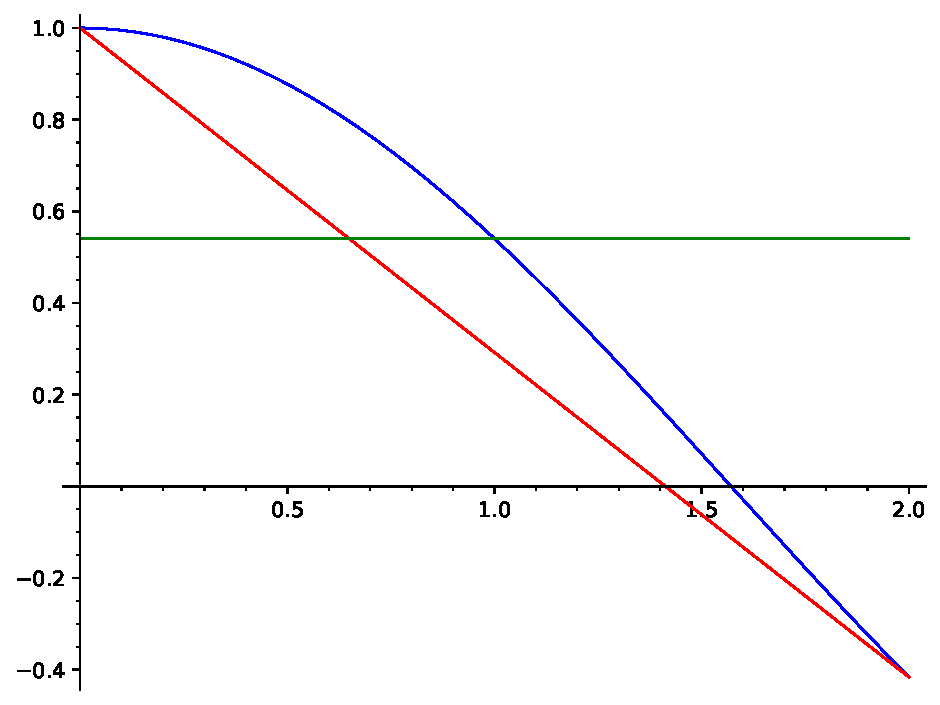
\includegraphics[height=30mm]{pics/plot_trapez.pdf}
	\begin{block}{Beispiel}
		\begin{itemize}
			\item Wir integrieren $f(x)=cos(x)$ auf dem Intervall $a=0$ bis $b=2$.
			\item Die analytische L\oe sung ist $\sin(2)\approx0.9093$.
			\item Approximation durch eine Konstante liefert $1.0806\cdots$.
			\item Die Trapezregel gibt $0.5839\cdots$.
		\end{itemize}
	\end{block}
\end{frame}

\begin{frame}\frametitle{\mytitle}
	\begin{block}{Fehlerterm der Trapezregel}
		\begin{itemize}
			\item Angenommen $f$ ist zweimal stetig differenzierbar.
			\item Dann gilt
				\begin{align*}
					\abs{\int_a^bf(x)\dd x-\frac{(b-a)(f(a)+f(b))}{2}}\leq\sup_{x\in[a,b]}\frac{(b-a)^3}{12}|f''(x)|.
				\end{align*}
		\end{itemize}
	\end{block}
\end{frame}

\begin{frame}\frametitle{\mytitle}
	\begin{block}{Simpsonregel}
		\begin{itemize}
			\item Wir approximieren des Integral durch
				\begin{align*}
					\frac{b-a}{6}\brk{f(a)+4f\bcfr{a+b}2+f(b)}
				\end{align*}
			\item Der Fehlerterm ist abzusch\ae tzen durch
				\begin{align*}
					\frac{(b-a)^5}{2880}\sup_{x\in[a,b]}|f''''(x)|.
				\end{align*}
				sofern $f$ viermal stetig differenzierbar ist.
		\end{itemize}
	\end{block}
\end{frame}

\begin{frame}\frametitle{\mytitle}
	\hfill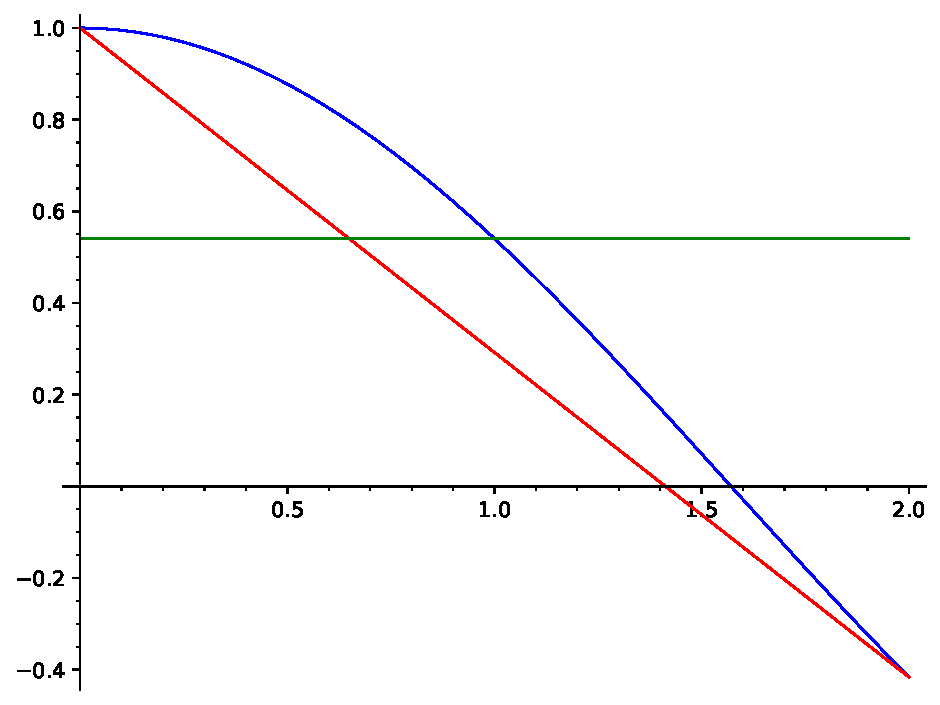
\includegraphics[height=30mm]{pics/plot_trapez.pdf}
	\begin{block}{Beispiel}
		\begin{itemize}
			\item Wiederum sei $f(x)=\cos(x)$ auf dem Intervall $a=0$ bis $b=2$.
			\item Die analytische L\oe sung ist $\sin(2)\approx0.9093$.
			\item Die Simpsonregel gibt $0.9150\cdots$.
		\end{itemize}
	\end{block}
\end{frame}

\begin{frame}\frametitle{\mytitle}
	\begin{block}{Newtonsche $\frac{3}{8}$-Regel}
		\begin{itemize}
			\item Wir approximieren des Integral durch
				\begin{align*}
					\frac{b-a}{8}\brk{f(a)+3f\bcfr{2a+b}3+3f\bcfr{a+2b}3+f(b)}.
				\end{align*}
			\item Der Fehlerterm ist abzusch\ae tzen durch
				\begin{align*}
					\frac{(b-a)^5}{6480}\sup_{x\in[a,b]}|f''''(x)|.
				\end{align*}
		\end{itemize}
	\end{block}
\end{frame}

\begin{frame}\frametitle{\mytitle}
	\hfill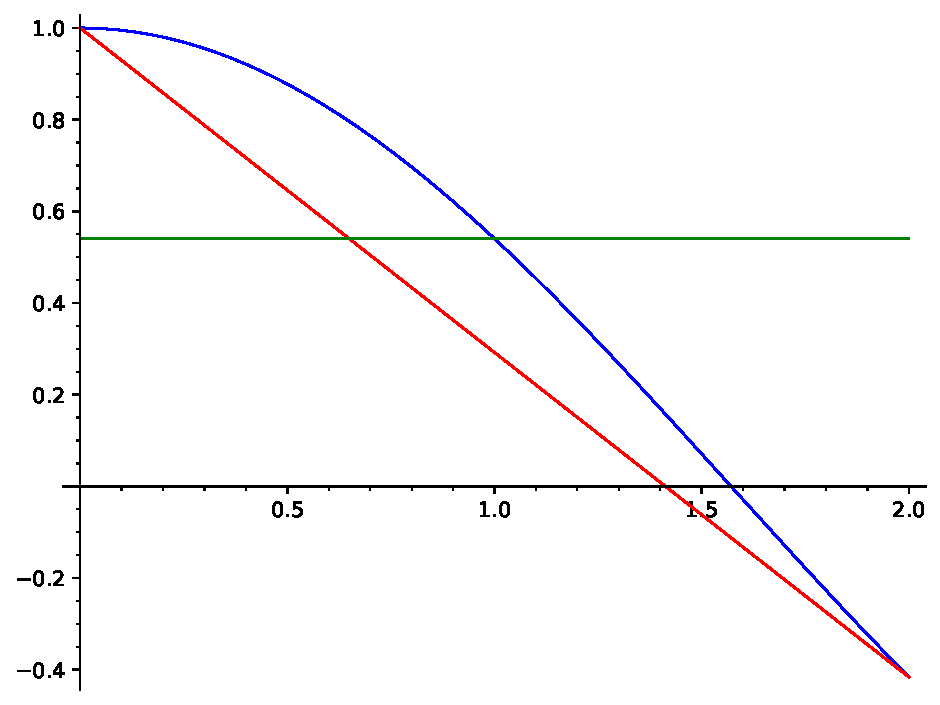
\includegraphics[height=30mm]{pics/plot_trapez.pdf}
	\begin{block}{Beispiel}
		\begin{itemize}
			\item Wiederum sei $f(x)=\cos(x)$ auf dem Intervall $a=0$ bis $b=2$.
			\item Die analytische L\oe sung ist $\sin(2)\approx0.9093$.
			\item Die Newtonsche $\frac{3}{8}$-Regel gibt $0.9118\cdots$.
		\end{itemize}
	\end{block}
\end{frame}

\begin{frame}\frametitle{\mytitle}
	\begin{block}{Milneregel oder Booleregel}
		\begin{itemize}
			\item Wir approximieren des Integral durch
				\begin{align*}
					\frac{b-a}{90}\brk{7f(a)+32f\bc{\frac{3a+b}{4}}+12f\bc{\frac{a+b}{2}}+32f\bc{\frac{a+3b}{4}}+7f(b)}
				\end{align*}
			\item Der Fehlerterm ist abzusch\ae tzen durch
				\begin{align*}
					\frac{(b-a)^5}{1935360}\sup_{x\in[a,b]}|f^{[6]}(x)|.
				\end{align*}
		\end{itemize}
	\end{block}
\end{frame}

\begin{frame}\frametitle{\mytitle}
	\hfill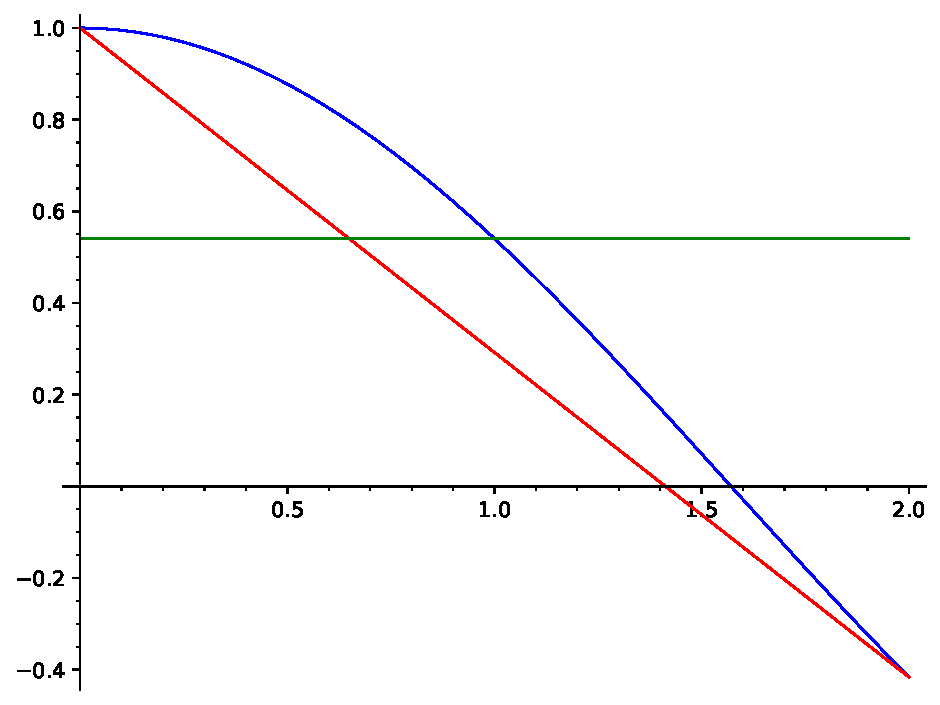
\includegraphics[height=30mm]{pics/plot_trapez.pdf}
	\begin{block}{Beispiel}
		\begin{itemize}
			\item Wiederum sei $f(x)=\cos(x)$ auf dem Intervall $a=0$ bis $b=2$.
			\item Die analytische L\oe sung ist $\sin(2)\approx0.9093$.
			\item Die Booleregel gibt $0.9093\cdots$.
		\end{itemize}
	\end{block}
\end{frame}

\begin{frame}\frametitle{\mytitle}
	\begin{block}{Die Newton-Cotes-Formeln}
		\begin{itemize}
			\item Wie k\oe nnen diese Formeln vereinheitlicht werden?
			\item F\ue r eine gegebene Ordnung $n\geq1$ setze
				\begin{align*}
					h&=\frac{b-a}{n}&&x_i=a+ih&(i=0,\ldots,n).
				\end{align*}
			\item Wir approximieren die Funktion $f$ durch die Lagrangepolynome an den Punkten $x_0,\ldots,x_n$ und integieren letztere analytisch.
			\item Dies f\ue hrt auf die Gewichte
				\begin{align*}
					w_i&=\frac{1}{b-a}\int_a^b\prod_{\substack{0\leq j\leq n\\j\neq i}}\frac{x-x_j}{x_i-x_j}\dd x
				\end{align*}
		\end{itemize}
	\end{block}
\end{frame}

\begin{frame}\frametitle{\mytitle}
	\begin{block}{Die Newton-Cotes-Formeln}
		\begin{itemize}
			\item Die obigen Integrationsformeln sind die Spezielf\ae lle $n=1,2,3,4$.
			\item F\ue r die Ordnungen $n=1,\ldots,7$ sind die Koeffizienten nicht-negativ.
			\item H\oe here Ordnungen sollten daher vermieden werden.
		\end{itemize}
	\end{block}
\end{frame}

\begin{frame}\frametitle{\mytitle}
	\begin{block}{Gau\ss quadratur}
		\begin{itemize}
			\item In den Newton-Cotes-Formeln haben wir die Funktion an \ae quidistanten Punkten ausgewertet.
			\item In der Gau\ss quadratur werden die Punkte, an denen die Funktion ausgewertet wird, zus\ae tzlich geschickt gew\ae hlt.
			\item Dadurch k\oe nnen Polynome bis zum Grad $2n-1$ durch Auswertung an $n$ Punkten exakt integriert werden.
			\item Die Gau\ss quadratur ist auch von Interesse, wenn der Integrand eine Produktform aufweist.
		\end{itemize}
	\end{block}
\end{frame}

\begin{frame}\frametitle{\mytitle}
	\begin{block}{Iterative Verfahren}
		\begin{itemize}
			\item Die obigen Formeln liefern nur eine begrenzte Genauigkeit.
			\item Diese kann verbessert werden, wenn der Integrationsbereich zerlegt wird:
				\begin{align*}
					\int_a^bf(x)\dd x=\int_a^cf(x)\dd x+\int_c^bf(x)\dd x.
				\end{align*}
			\item Die Unterteilung kann wiederholt werden.
		\end{itemize}
	\end{block}
\end{frame}

\begin{frame}\frametitle{\mytitle}
	\begin{block}{Adaptive Verfahren}
		\begin{itemize}
			\item Moderne numerische Integrationsverfahren verwenden eine adaptive Zerlegung des Integrationsbereichs.
			\item Die Details \ue bersteigen den Rahmen dieser Vorlesung.
			\item Die numerische Quadratur ist ein Spezialfall der Numerik von Differentialgleichungen.
		\end{itemize}
	\end{block}
\end{frame}

\begin{frame}\frametitle{\mytitle}
	\begin{block}{Zusammenfassung}
		\begin{itemize}
			\item Numerische Quadraturverfahren erm\oe glichen die n\ae herungswiese Berechnung von Integralen.
			\item Wir haben mehrere Integrationsformeln kennengelernt; viele davon sind Spezielf\ae lle der Newton-Cotes-Formeln.
			\item F\ue r hinreichend glatte Funktionen kann die Genauigkeit quantifiziert werden.
		\end{itemize}
	\end{block}
\end{frame}
\end{document}
